\chapter{Desarrollo de prototipos}
\label{cap:Desarrollo de prototipos}


%PRIMERA VERSIÓN EN BARD
%PRIMERA VERSIÓN EN GEMMA
%PRIMERA VERSIÓN GEMINI - GOOGLE COLLABORATE
%REFACTORIZACIÓN PARA HACER VERSIÓN LOCAL
%TELEGRAM
%GENERAR LAS ETAPAS 
%IMAGENES
%WHISPER
%GRÁFOS
%GENERACIÓN DE HISTORIAS DE VIDA
El capítulo actual tiene como objetivo presentar en orden temporal los distintos prototipos que se han desarrollado hasta llegar a la versión final que se presenta en el capítulo \ref{cap:ChatBot final}. 

La estructura del capítulo  muestra en orden lineal en el tiempo como se ha ido construyendo la arquitectura del sistema. De esta forma se puede ver como el modelo va pasando por distintos prototipos de forma incremental. 

En este capítulo, también se pretende mostrar y hacer hincapié en los diferentes desafíos, contratiempos y retos a los que ha habido qué hacer frente durante el desarrollo del prototipo, por qué se han originado y cómo se han solucionado. 

Con todo ello, se pretende tener una visión global de lo que ha sido el trabajo de desarrollo del sistema. Partiendo de la situación que se muestra en el capítulo \ref{cap:estadoDeLaCuestion}, con el estudio teórico llevado a cabo en el capítulo \ref{cap:TecnologiasUtilizadas} y dando lugar al sistema que se detallará en el capítulo \ref{cap:ChatBot final}. 

El código asociado a los distintos prototipos se puede consultar en el repositorio de GitHub, y en concreto, en la carpeta de prototipos. 

\section{Planteamiento del problema}
Cómo se comento en el capítulo \ref{cap:introduccion}, el objetivo de este proyecto es construir una herramienta que fácilite a los terapeutas la labor de realizar terapias de reminiscencia a personas con demencia. Para ello, se trata de obtener un chatbot capaz de realizar preguntas adecuadas, extraer información útil de ellas y generar nuevas preguntas para rellenar la información faltante. 

Con este objetivo en mente, se plantea un diseño iterativo que parta de un chatbot capaz de realizar preguntas predefinidas y sobre él ir iterando hasta conseguir un prototipo completo.
\section{Preguntas predefinidas y análisis de las respuestas usando BARD}
\label{sec:prototipoBARD}
La primera versión del prototipo tuvo como único objetivo ser una herramienta capaz de realizar una serie de preguntas predefinidas, y almacenar la información obtenida.

Para el almacenamiento de la información se decidió usar \textit{JSON} debido a su estructura legible y su amplia compatibilidad, suponen una elección tecnológica ideal para almacenar los datos de este sistema.Su capacidad para representar datos complejos de manera eficiente y su interoperabilidad garantizan una experiencia de desarrollo ágil y una gestión eficaz de la información de los usuarios. 

Por otro lado, se desarrollo una pequeña clase de forma provisional. Esta clase es la clase \textit{Paciente} que tenía como objetivo estructurar y reunificar la información.

A continuación, se busco poder hacer un análisis de las respuestas exhaustivo que permitiera extraer información útil de las respuestas dadas por el usuario.

Tras el estudio realizado en la sección \ref{sec:apis} se tomo la decisión de utilizar la API de BARD. Las principal característica que llevo a tomar esta decisión es que se trata de una API ya entrenada capaz de crear texto de alta calidad similar al humano. Está hecha a medida para desarrolladores y creadores de contenidos, permitiendo la automatización de la generación de contenidos para diversas necesidades, como en este caso la generación de un chatbot. Todo esto, supone una gran ventaja frente a otras herramientas como las distintas bibliotecas que suponen desarrollar y generar nuestros propios algoritmos de generación del lenguaje, o otras APIs que requieren un entrenamiento que da lugar a horas y horas de computo para obtener resultados, a lo sumo, tan buenos como los que ofrecía BARD con su simple instalación. 

Para instalar BARD se utilizo el entorno de \textit{Google Collaborate}. En primer, lugar fue necesario instalar los paquetes \textit{bardapi} y \textit{pyTelegramBotApi}. Una vez intaladas las bibliotecas y para usar la API es necesario registrarse y obtener un token que nos sirve como identificador de la API. 

Una vez con todo instalado, se utilizó la API Bard para extraer información a partir de respuestas a preguntas específicas. 
\begin{figure}[h]
	\centering
	\begin{verbatim}
		prompt = "A partir del texto a continuación, que contiene información
		sobre una persona y damelo en una lista info donde
		info[nombre]:valor_atributo.  Limitate a dar la información pedida. "
		
		texto = "Hola mi nombre es Marta, tengo 22 años y soy de Zaragoza."
		>> **Info[nombre:Marta;edad:22;ciudad:Zaragoza]** 
		¿Hay algo más que pueda hacer por ti?
	\end{verbatim}
	\caption{ Ejemplo de uso de BARD.}
	\label{fig:ejemploBARD}
\end{figure}
Como se ve en la figura \ref{fig:ejemploBARD}, BARD supone una herramienta útil para la extracción de información a partir de respuestas y la estructuración de la misma. Sin embargo, aunque indiques que se limite a darte la información pedida, en una amplio número de casos añade texto adicional como en este caso \textit{``¿Hay algo más que pueda hacer por ti.''}. Para corregir esto se desarrolló una serie de funciones que parsearan el texto de forma manual, a partir de la respuesta dada por BARD. En concreto, la función $extraer\_info$ que extrae información de un texto en un formato específico, que es el pedido a BARD, y la devuelve como un diccionario de atributo-valor. Por otro lado, la función $parsear\_info$ procesa la información proporcionada por el usuario y actualiza el objeto paciente. 

La interacción chatbot usuario de este prototipo se llevaba a cabo mediante una pequeña interfaz desarrollada con widgets de IPyhton. 
Esta versión del chatbot solicita al usuario información como nombre, edad, ciudad, etc., y al final muestra un mensaje de despedida con los datos recopilados.
\begin{figure}[h]
	\centering
	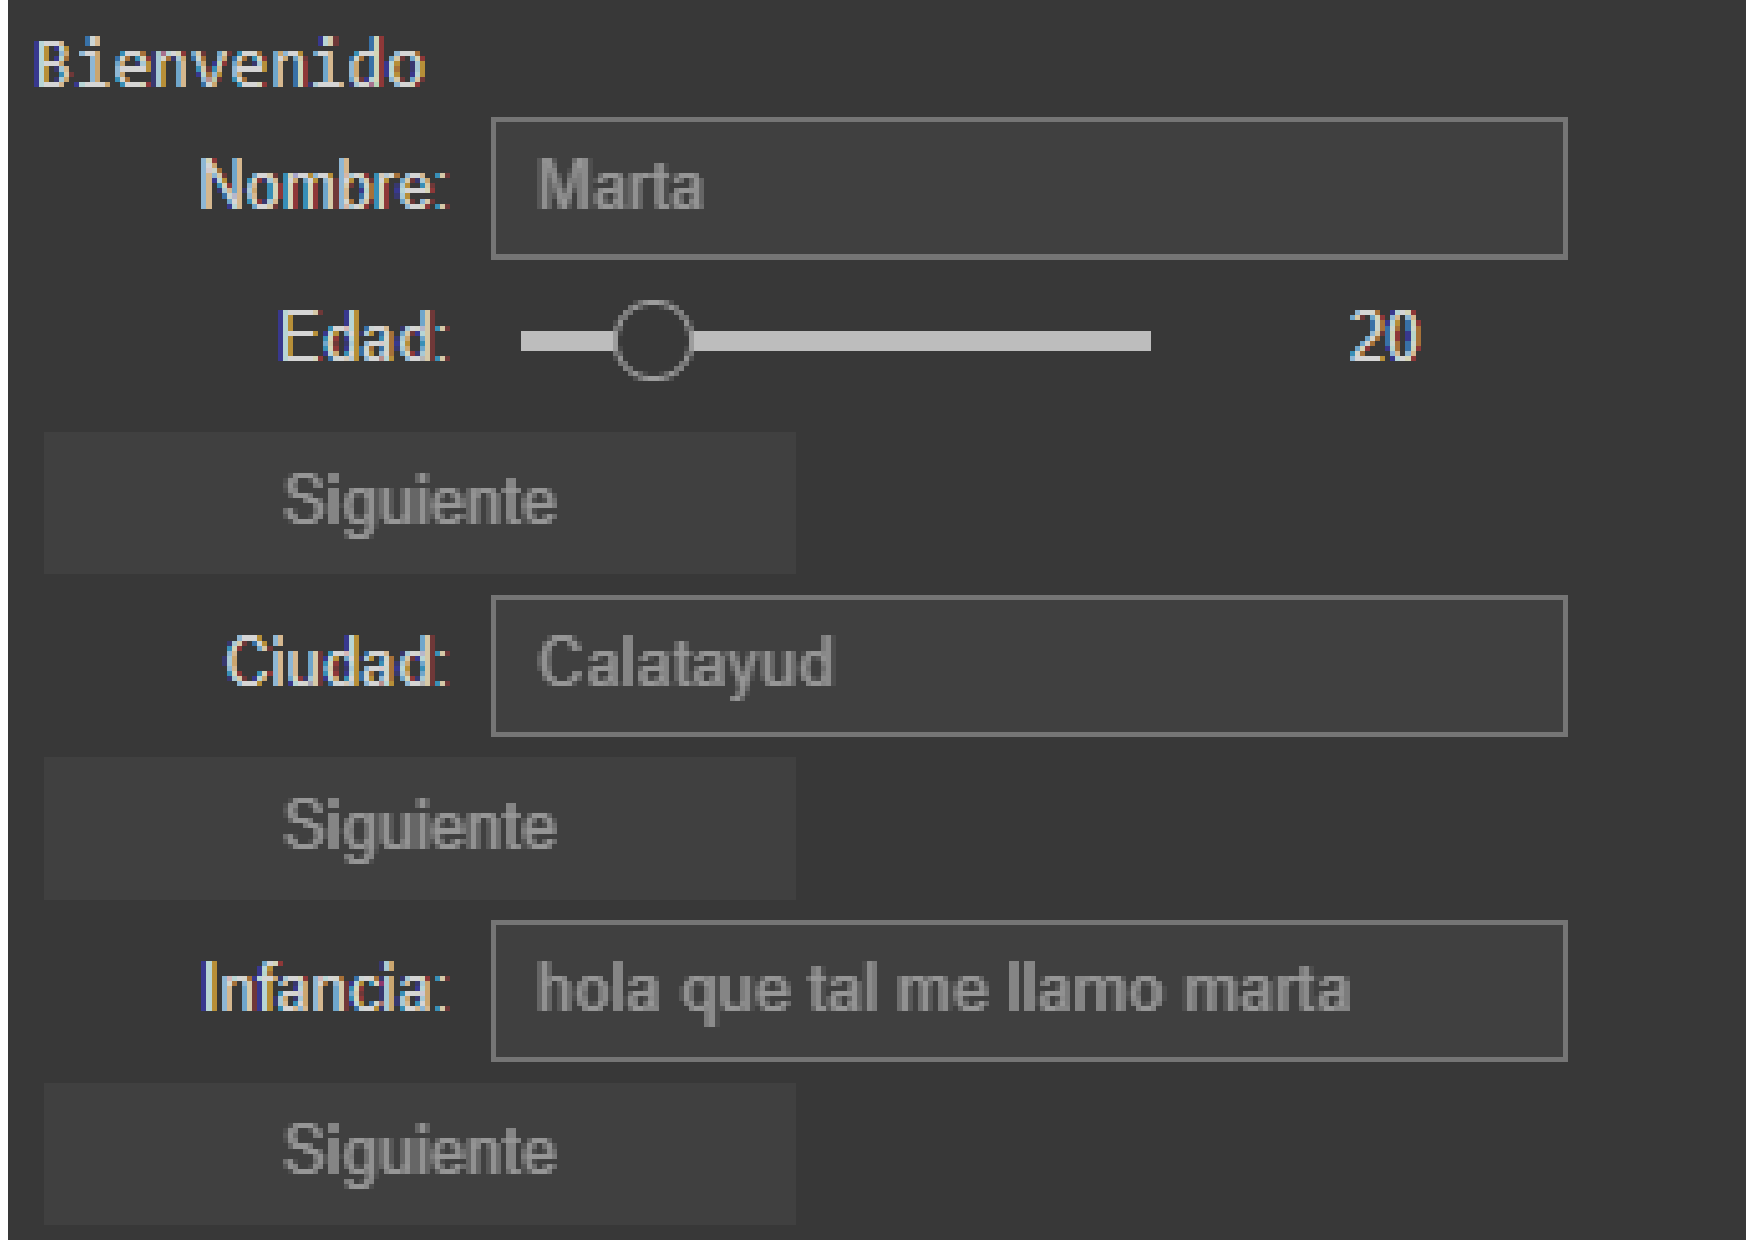
\includegraphics[width=0.5\textwidth]{Imagenes/Iwidget}
	\caption{Muestra de la interacción chatbot-usuario en el primer prototipo}
	\label{fig:interfazPrototipo1}
\end{figure}
Cómo se puede ver en la figura \ref{fig:interfazPrototipo1}, la interacción con el usuario se hace mediante cajas en las que se escribe la información solicitada. Una vez rellanado se envía la información al chatbot para su análisis pulsando en el botón ``Siguiente'' que despliega un nuevo cuadro con la siguiente información solicitada. 

Todo este desarrollo se llevo a cabo durante en los meses previos a diciembre de 2023. Fue ese mes cuando Google fortaleció la capacidad de Bard brindando habilidades más avanzadas de comprensión, razonamiento, resumen y codificación. De esta forma, paso a ser Gemini. Este cambio se oficializo en Febrero de 2024 y supuso la imposibilidad de usar BARD debido a las restricciones de uso según la localización de Gemini. Esta restricción limita el uso de la API de Gemini a una serie de regiones entre las que no se encuentra España ni ningún país de la Unión Europea.

En consecuencia, este primer prototipo paso a un segundo plano y se centro el trabajo de los siguientes meses en encontrar qué API usar para el desarrollo del trabajo. Se barajaron distintas posibilidades. 

Por un lado se estudio la API de GPT por sus buenas prestaciones y características, ya presentadas en el capítulo \ref{cap:TecnologiasUtilizadas}. Sin embargo, la API es de pago y para usarla en las versiones de bajo precio o gratuito es recomendable entrenarlo lo que suponía un coste en computo no asumible. 

Por otro lado , se decidió estudiar distintos modelos de hugging face \footnote{https://huggingface.co/} entre los que destaco gemma. 

\section{Prototipo usando GEMMA}
Al comenzar a desasrrollar este prototipo, se trató de seguir una estructura que permitiera reutilizar todo el código posible del prototipo anterior. Para ello, se trato de desarrollar una versión de nuevo en $Google Collaborate$. Posteriormente, se estudió la alternativa de la implementación de un modelo local. En el desarrollo de este prototipo se utilizaron diferentes bibliotecas de $Hugging Face$.

\texttt{AutoTokenizer} y \texttt{AutoModelForCausalLM} son clases proporcionadas por la biblioteca $Hugging Face Transformers$ que se utilizan para cargar y trabajar con modelos de lenguaje preentrenados.

\begin{enumerate}
	\item \texttt{AutoTokenizer}: Esta clase se utiliza para cargar un tokenizador adecuado para el modelo de lenguaje preentrenado que se desea utilizar. El tokenizador se encarga de dividir el texto en unidades más pequeñas, como palabras o subpalabras, y convertirlas en vectores numéricos que el modelo de lenguaje puede entender. En nuestro contexto 
	
\begin{verbatim}
AutoTokenizer.from_pretrained(``google/gemma-7b'')
\end{verbatim}

se utiliza para cargar el tokenizador asociado al modelo de lenguaje $gemma-7b$ de Google.
	
	\item \texttt{AutoModelForCausalLM}: Esta clase se utiliza para cargar el modelo de lenguaje preentrenado que se desea utilizar. El modelo de lenguaje es responsable de generar texto basado en las entradas proporcionadas. En nuestro contexto,
\begin{verbatim}
AutoModelForCausalLM.from_pretrained(''google/gemma-7b´´)
\end{verbatim}
	
se utiliza para cargar el modelo de lenguaje "gemma-7b" de Google, que es capaz de generar texto de manera condicional, es decir, generar texto secuencialmente teniendo en cuenta el contexto anterior.
\end{enumerate}

En resumen, utilizaremos \texttt{AutoTokenizer} para cargar el tokenizador asociado al modelo de lenguaje preentrenado, y \texttt{AutoModelForCausalLM} para cargar el propio modelo. Estas clases son esenciales para preparar el modelo para su uso en la generación de texto o en otras tareas de procesamiento de lenguaje natural.

\subsection{Google Collaborate}
En primer lugar, para poder descargarnos el modelo se tiene que utilizar la biblioteca ``os'' para establecer las credenciales de autenticación de Hugging Face. Esto es necesario para acceder a modelos alojados en $Hugging Face$ y para realizar operaciones como clonar repositorios de modelos.

A continuación es necesaria la carga de la clase ``AutoTokenizer'' y ``AutoModelForCausalLM'' de la biblioteca ``Transformers'' de Hugging Face para cargar un tokenizador y un modelo de lenguaje preentrenado. En este caso, el tokenizador y el modelo elegidos se cargan desde la dirección $``google/gemma-7b''$. 

Para poder realizar todas estas instalaciones se ha de configurar el entorno de ejecución de $Google Collaborate$ de forma que se utilicen cuatro GPUs. Esto requiere seleccionar la versión ``T4 GPU'' del acelerador de hardware. Ejecutar el programa sin seleccionar esta opción impedimenta la carga y descarga de los modelos y el programa y en consecuencia su uso. 

Una vez realizada toda esta instalación, se puede utilizar el modelo de lenguaje cargado para generar texto a partir de una entrada específica. Sin embargo, en su versión gratuita $Collaborate$ tiene limitado el uso de varios GPUs con lo que esta versión apenas pudo ser usada antes de que el entorno de ejecución limitara el uso de más de una GPU y en consecuencia, hubiera que descartar la alternativa de seguir desarrollando con $gemma-7$ en $Collaborate$.

En resumen, este código carga un modelo de lenguaje preentrenado, genera texto utilizando el modelo y realiza operaciones relacionadas con la gestión de modelos alojados en $Hugging Face$.

\subsection{Linux}
Las versiones locales de $gemma-2b$ y $gemma-7b$ en local han de ser instaladas en Linux debido a sus características. Requiere la instalación de las bibliotecas comentadas anteriormente así como de $Hugging Face$ para poder acceder a los modelos. 

En primer lugar, se opto por el modelo $gemma-2b$ pero debido a las limitaciones del mismo y a la alta exigencia de las tareas que se requieren en este proyecto, se tuvo que usar el modelo de 7 millones de parámetros. Con él, se llego a implementar una versión similar a la descrita en la sección \ref{sec:prototipoBARD} pero mediante el uso de $gemma-7b$ de $Hugging Face$. 

Se amplió este modelo, tratando de alcanzar el siguiente reto: la generación de preguntas. Para ello, se desarrollo un módulo de generación de preguntas.

El módulo en concreto aborda la tarea de generar preguntas a partir de un texto dado utilizando herramientas de procesamiento de lenguaje natural. En concreto, se centra en la biblioteca $spaCy$, una poderosa herramienta para el procesamiento avanzado del lenguaje natural que ya ha sido presentada en la sección \ref{sec:Spacy} .

La generación de preguntas comienza con la tokenización y el análisis sintáctico del texto proporcionado. Para este propósito, se utiliza el modelo preentrenado de $spaCy$ en español, denominado \textit{$``es\_core\_news\_sm''$}. Este modelo es capaz de analizar la estructura gramatical del texto y etiquetar cada token con información como el tipo de palabra (sustantivo, verbo, etc.) y la categoría gramatical.

Una vez que el texto ha sido analizado, el módulo procede a identificar los sustantivos dentro del texto. Esto se logra mediante el análisis de las etiquetas gramaticales asignadas por $spaCy$ a cada token. Cada sustantivo identificado se considera como un tema potencial para formular preguntas.

Con los sustantivos identificados, el módulo genera preguntas sobre la experiencia relacionada con cada uno de ellos. Por ejemplo, si el texto menciona la palabra es ``viaje'', el módulo formulará la pregunta ``¿Qué tal tu experiencia de viaje?''.

Para el desarrollo de la interfaz de usuario, se consideraron dos enfoques diferentes: uno utilizando el framework Flask para crear un servidor web y otro utilizando la biblioteca Tkinter para construir una interfaz gráfica de usuario (GUI) de escritorio.

Con Flask, se optó por crear un servidor web que presenta una página web con un formulario. Flask maneja las rutas y funciones asociadas, permitiendo que los usuarios ingresen información en el formulario y envíen los datos al servidor. Esto resulta en una interfaz basada en la web que puede ser accesible a través de un navegador.

Por otro lado, con Tkinter, se creó una interfaz gráfica de usuario (GUI) de escritorio. Tkinter permite crear ventanas, etiquetas y botones para construir la interfaz. En este caso, se diseñó una ventana con una etiqueta de pregunta y dos botones de opción (``Sí'' y ``No''). Esta interfaz se ejecuta localmente en la máquina del usuario y es independiente del navegador web.

Este prototipo que supone un incremento respecto al anterior también tuvo que ser descartado sin llegar a desarrollar algunas funcionalidades y módulos hasta el final, como por ejemplo la interfaz o la generación de preguntas. Este parón se debió a un problema hardware. Al hacer instalarme Linux, no tenía apenas espacio en el disco duro por lo que la partición no fue demasiado grande. El gran tamaño de los modelos, en concreto del modelo $gemma-7b$ ocupó gran parte del espacio de la partición. Pocas semanas después del comienzo del desarrollo de este prototipo tuvo que descartarse debido a la necesidad de ejecutarlo en Linux, acompañada de las limitaciones de espacio en mi ordenador que hicieron que no pudiera seguir desarrollandolo en ese sistema operativo. 

\section{Desarrollo de la interfaz con RASA}
Paralelamente a todo el trabajo descrito anteriormente, y durante el estudio de las diferentes alternativas de interfaces, APIs y modelos se estudio la alternativa de la api de rasa de la que ya se ha hablado en la sección \ref{subsec:rasa}. 

Esta opción fue inicialmente barajada como alternativa a BARD o Gemma, sin embargo, su capacidad de generación de texto no cumplía los requisitos requeridos para este proyecto por lo que se descarto para tal uso. 

Sin embargo, se encontró especialmente interesante debido a su fácil integración con Telegram para desarrollar chatbots. Como se puede ver en la figura \ref{fig:ejemploRASATELEGRAM} la interfaz generada de esta forma presenta númerosas ventajas. 

En primer lugar, Telegram es una plataforma de mensajería ampliamente utilizada en todo el mundo, lo que garantiza un amplio alcance y accesibilidad para los usuarios. Esto significa que los usuarios pueden acceder al chatbot fácilmente desde su escritorio, pero también desde sus dispositivos móviles, lo que facilita su adopción y uso.

\begin{figure}[h]
	\centering
	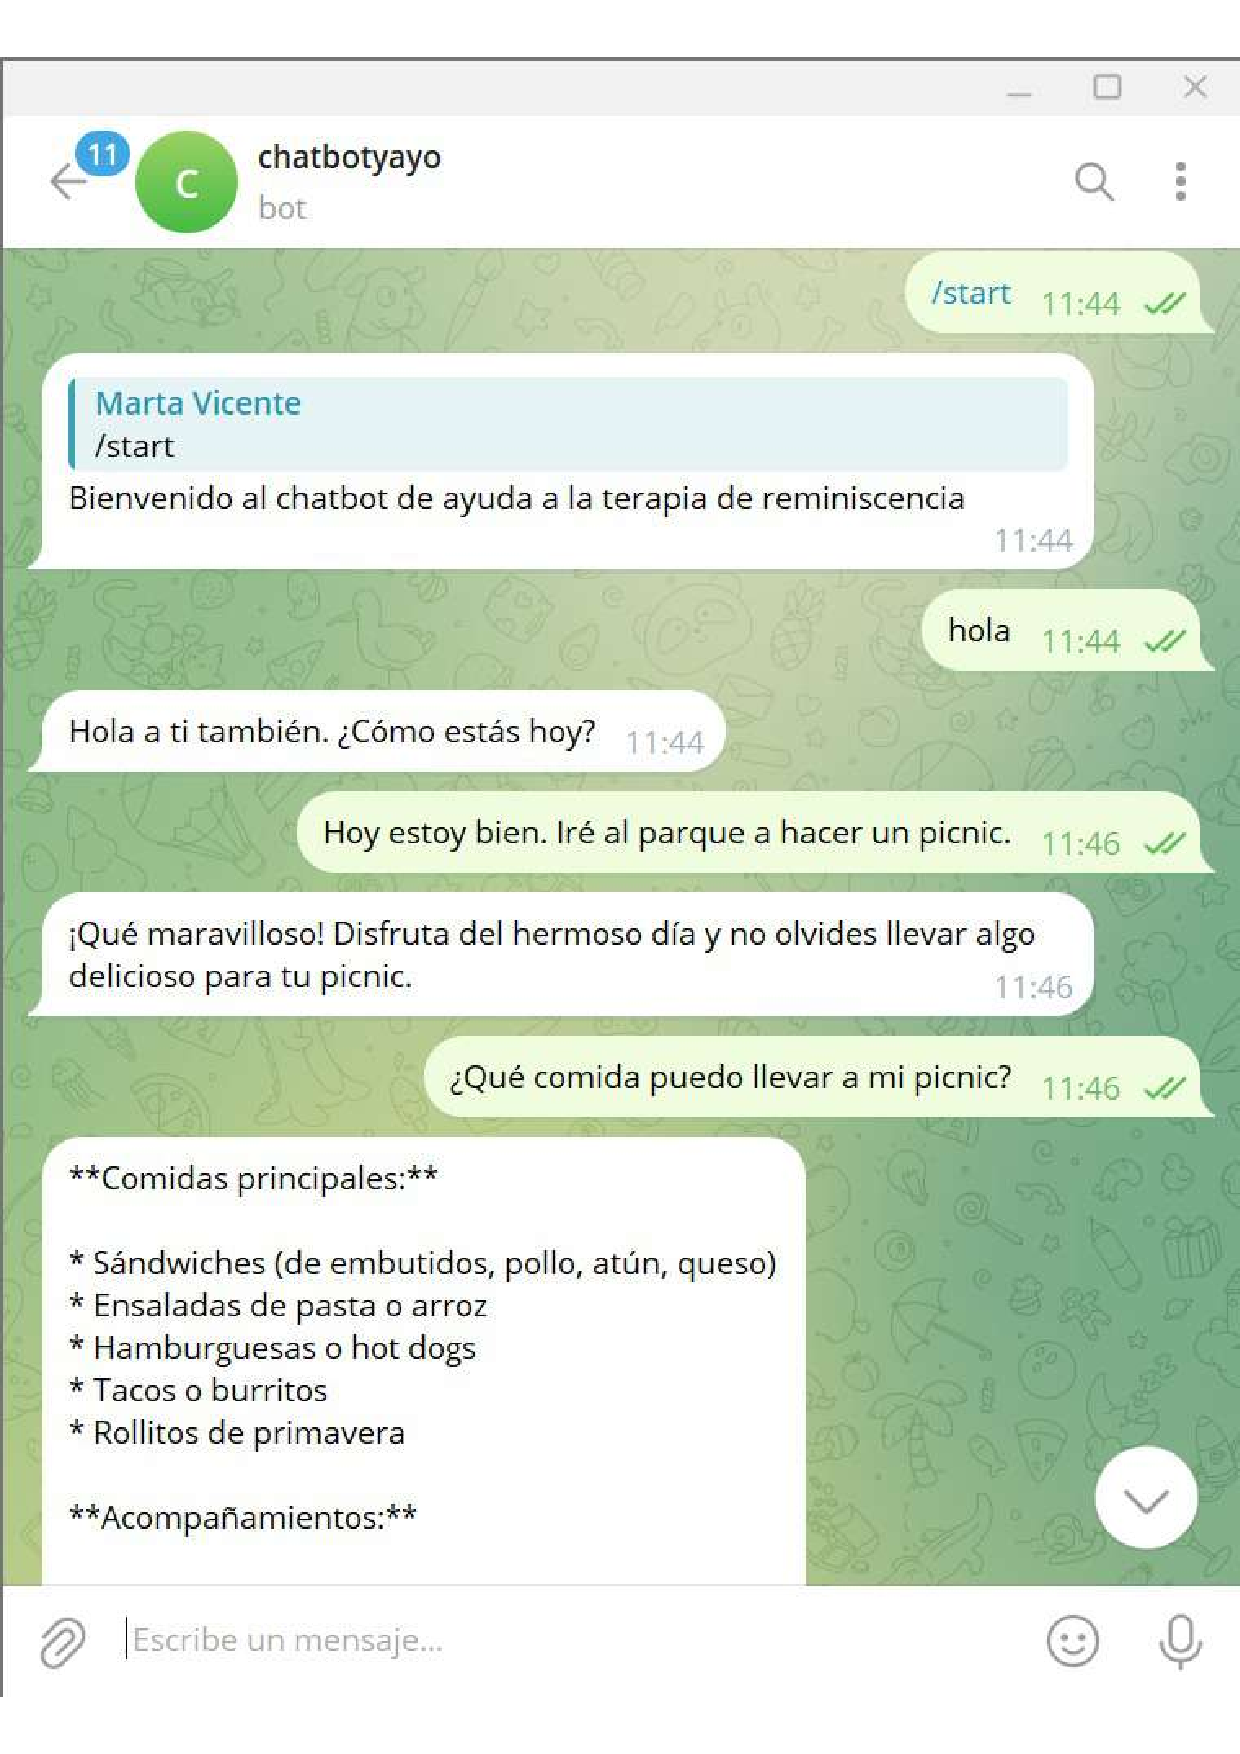
\includegraphics[width=0.5\textwidth]{Imagenes/telegram1}
	\caption{ Ejemplo de uso de BARD.}
	\label{fig:ejemploRASATELEGRAM}
\end{figure}

Esta forma de generar la interfaz implica el desarrollo de manejadores que controlen el funcionamiento según el tipo de mensaje. 
	
\begin{itemize}
	\item Manejadores para comandos, por ejemplo, el comando start.
	
	\item Manejadores para mensajes de texto.
	
	\item Manejadores para imagenes. 
\end{itemize}
	
Se utiliza la API de Telegram a través del módulo ``telebot'' para interactuar con el servicio de mensajería y gestionar los mensajes entrantes y salientes. Además, se inicia un bucle de escucha para que el bot esté constantemente activo y pueda responder a los mensajes de los usuarios en tiempo real.

\section{Gemini}
A lo largo de los meses se estudiaron múltiples modelos y alternativas a BARD que no resultaban lo suficientemente eficaces. Por contrario, otras sí resultaron eficaces y pese a dar lugar a pequeños prototipos no pudieron seguir desarrollandose debido a los diversos problemas que se han contado a lo largo de este capítulo. Todo este estudio, implementación de modelos y desarrollo de prototipos fallidos conlleva horas de tiempo y esfuerzo. Todo esto deriva en meses centrados en análisis de alternativas en lugar del propio desarrollo del código en sí, por lo que finalmente hubo que decantarse por la API que resultaba más eficaz y fiable y que daba mejores resultados: la API de Gemin. Como se ha comentado antes, esta alternativa se descarto en un primer momento por no estar disponible en España. Sin embargo este problema se pudo solventar fácilmente mediante el uso de VPN.
%API DE GEMINI
%VPN 
%VERSIÓN COLLABORATE
%VERSIÓN LOCAL 


\section{Selección de las preguntas predefinidas}
Para la selección de las preguntas predefinidas he optado por emplear la plantilla ``Life History Templates'' \cite{DUK89b}. Estas preguntas desempeñan un papel crucial en el flujo de interacción del sistema, ya que son el esqueleto principal de la conversación con el usuario. 

La plantilla \cite{DUK89b}, concebida con el propósito de estructurar la recopilación de información sobre la historia de vida de un individuo, ofrece una serie de campos predefinidos que abarcan una amplia gama de aspectos relevantes. Dichos campos han sido seleccionados, con el objetivo de garantizar una exploración exhaustiva y completa de la vida del paciente tratando de asegurar que se aborden aspectos clave de la vida del paciente, tales como eventos significativos, relaciones personales, intereses y preferencias, entre otros. Esto permite obtener una visión completa y detallada del individuo, lo cual es fundamental para proporcionar una atención personalizada y efectiva.

Una vez que se han identificado los campos pertinentes, se procede a la creación de un documento denominado ``preguntas.txt'', el cual sirve como guía durante la interacción con el paciente. En este documento se registran las preguntas específicas que se deben realizar en cada campo, así como la información deseada que se espera obtener a través de las respuestas del paciente. Esto facilita el seguimiento y la organización de la información recopilada, asegurando que se cubran todos los aspectos relevantes de la historia de vida del individuo.

Además, la plantilla ``Life History Templates'' incluye la recomendación de utilizar fotografías como herramienta para estimular la memoria y facilitar la obtención de información por parte del paciente. Esta estrategia, basada en la estimulación visual, ha demostrado ser efectiva para desencadenar recuerdos y promover la narración de experiencias pasadas.

Como parte de la implementación de nuestro prototipo, planeamos integrar esta funcionalidad en la sección dedicada a las imágenes (sección \ref{sec:imagenes}). Esto permitirá enriquecer la interacción con el paciente y mejorar la calidad de la información recopilada, contribuyendo así a una evaluación más completa y precisa de su historia de vida. 

\section{Clase Pregunta}
\subsection{Análisis de las respuestas con Gemini}

%Cuándo las preguntas son de si o no hay que hacer un tratamiento diferente puesto que si no la api se lia. 
\subsection{Generación de preguntas con Gemini}
\subsection{Almacenamiento de la información}
\section{Integración de Gemini y RASA}
%Para poder hacer la refactorización y guardar toda la información se crea la clase pregunta, que hace que se refactorice todo  demás 

\section{Extracción de información a partir de imagenes}
\label{sec:imagenes}

\section{Gemini almacenamiento de información}
Como se puede ver en la figura \ref{fig:interfazPYQT5} estas bibliotecas permiten crear interfaces bastantes usables y simples. Sin embargo, aunque la interfaz es de buena calidad, se han explorado otras alternativas con el objetivo de obtener una interfaz 


